\documentclass[12pt]{article}
\usepackage{graphicx}
\usepackage{amsmath}
\usepackage{amssymb}
\usepackage{amstext}
\usepackage{amsfonts}
\usepackage{mathrsfs}
\usepackage{makeidx}
\usepackage{multirow}
\usepackage{pgfplots }
\setlength{\parindent}{0pt}
\title{STEM Gender Gap in University Education}
\date{June 2017}
\author{Peter Pointner ,Thomas Sulzbacher, Yang Hua}

\begin{document}
	\pagenumbering{gobble}
	\maketitle
	\newpage
	
	\tableofcontents
	\newpage
	\pagenumbering{arabic}
	\section{Abstract}
In this paper our team focuses on the gender gap which appears in Science Technology Engineering Mathematics and Computer ,henceforth STEM, majors in university education. First of all we want to give an overview of the current situation of inscription rates in different STEM related majors at Johannes Kepler University Linz, from now on  JKU, and how the development progressed from 2002 to 2016 based on \cite{studienwahl_jku} \cite{eq_1} \cite{eq_2} \cite{eq_3}. After taking a close look at the situation in Austria we want to focus on reasons for the decision made when choosing a university major and what different influences people are committed.
In the next section the gender gap in STEM majors on universities in Germany is evaluated and compared against the situation in Austria. The main focus ,of the second part of this report, is to take a closer look at the international situation of the STEM gender gap. At the end of the report a conclusion of our findings will be presented.    
 	\section{Situation in German speaking countries}
	\subsection{Situation at JKU}
The study conducted in  \cite{eq_1}\cite{eq_2}\cite{eq_3}  showed that from 2005 throughout 2016 the share between man and women studying at JKU was not reflecting the demographic composition of Austria which would be 51\% women and 49\% of men studying at JKU. In 2005  the share between man and women studying at JKU was at a rate of  45\% but there is a slight increase since 2005 to 2016 where 49\% of all students at JKU were female students. If a closer look is taken at the inscription rates of new students, the rate of women starting at JKU in 2016, we see that the share of women is 53\%, which also represents the mean of female students of all Austrian universities. From the gender equality reports conducted from 2005 to 2016 it can be seen that JKU has a general problem in attracting women but the problem minimized during the past years. \newline\newline
After describing the general share of female and male students at JKU a closer look is now taken at the STEM related majors.
Unfortunately the data presented in \cite{eq_1}\cite{eq_2}\cite{eq_3} is inconsistent with each other meaning some data given in \cite{eq_1}can not be found in \cite{eq_2} and \cite{eq_3} or is structured in a different way. First we want to take a look at the statistics for the whole Technical faculty of Natural Science, hence TNF.\newline
\begin{figure}[h!]
\centering
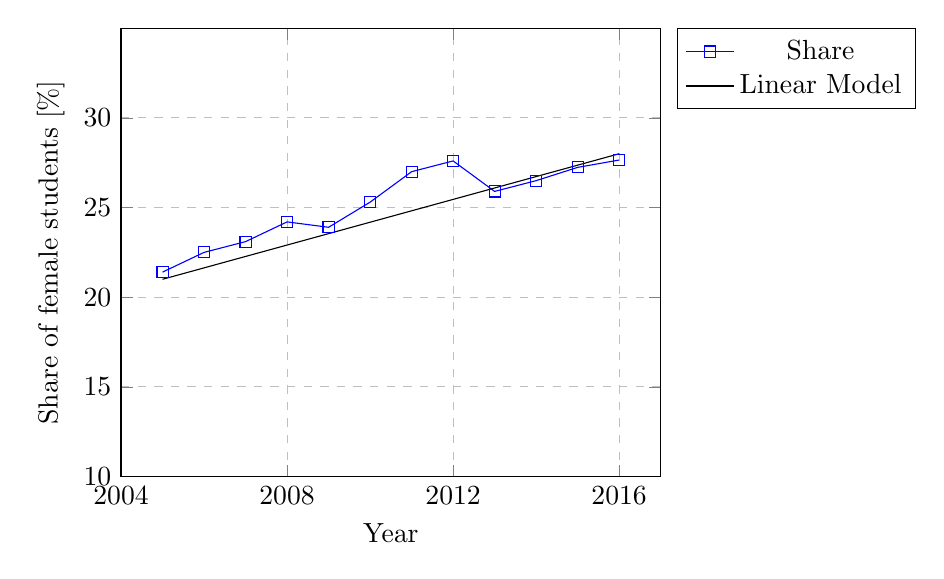
\begin{tikzpicture}
\begin{axis}[
    %title={STEM Gender Gap developement at JKU's TNF},
    	x tick label style={/pgf/number format/1000 sep=},
	xlabel={Year},
    	ylabel={Share of female students [\%]},
    	xmin=2004, xmax=2017,
    	ymin=10, ymax=35,
    	xtick={2004,2008,2012,2016},
    	ytick={0,10,15,20,25,30},
    	ymajorgrids=true,
	xmajorgrids=true,
    	grid style=dashed,
legend pos = outer north east,
]
\addplot[color=blue,mark=square,]
    coordinates {(2005,21.4)(2006,22.5)(2007,23.1)(2008,24.2)(2009,23.9)(2010,25.3)(2011,27.0)(2012,27.6)(2013,25.9)(2014,26.5)(2015,27.24)(2016,27.65)};
\addplot[color=black,mark=point,]
    coordinates {(2005,21)(2016,28)};
\legend{Share,Linear Model}
\end{axis}
\end{tikzpicture}
\caption[Developement of STEM Gap at JKU]{STEM Gender Gap developement at JKU's TNF.}
\label{fig:dev}
\end{figure}
In figure number \ref{fig:dev} we can see the development of the STEM Gap at JKU's TNF over a period of 11 Years. If   a linear regression model is assigned to the data ,given by the equality reports, with 
\begin{equation}
y= \frac{7}{11}*x+21.4
\end{equation}  we see that the slight increase of female students at JKU fits the chosen model pretty well and this model might be useful for further estimates of the general decrease of the STEM Gender Gap.
If we take a closer look on the different STEM topics we notice that the STEM Gap is not found in all majors. In general it can be said that the share of male and female students in majors having a bio-science background   is dominated by female students. The share is about 63\% and keeps steady over the years. 
The highest gap which can be found at JKU is in Computer Science with only a share of 13\% female students. If the data of the equality reports is analyzed in further detail it can be seen that there is also no increase of female students in Computer Science since 2005. In the section \ref{theories} theories for the occurrence of the STEM Gender Gap in University Education, especially in Computer Science, will be presented.
\subsection {Differences between Master and Bachelor Studies}
Unfortunately the data given by \cite{eq_1}\cite{eq_2}\cite{eq_3} is inconsistent in this point. In \cite{eq_1}and in \cite{eq_2} only PHD studies are separated from its predecessors meaning further analysis between Bachelor and Master programs is not possible. In \cite{eq_3} the distinction between the different stages is available and shows that the share of women is slightly decreasing between Bachelor and Master studies. This comparison can be performed for all studies except for studies related to Bio-science since the data given in that section is not realistic (8/15 people in Bachelors program, 17/31 Masters program and 332/162 PHD program) and needs to be clarified with the authors of the report. 
\subsection{Situation in Germany}
After the situation at Johannes Kepler University was evaluated in detail we want to take a closer look at the STEM Gender Gap in University Education in Germany based on \cite{schneider}. The statistics show that the share between female and male students is similar to the share in Austria. In Mathematics and Science related studies female students hold a quota of about  37\% in Engineering and Computer Science Related topic the ratio drops to around 21\% female students in total. Studies performed by the German Government show that there is a constant increase of female students in STEM related studies since 1995. This constant increase can also be monitored in Austria as the graph in \ref{fig:dev} shows.\newline
The statistics mentioned in \cite{schneider} also mention that the drop out rate of male students is relatively higher for boys than for girls, meaning when women decide to study a STEM major the chances are higher they will stick with their choice than men. The ratio of drop out rates is in general high in STEM majors with 42\% of female students drop out rate and a drop out rate of 49\% for male students.
Another interesting finding is that the share of graduations for female students is rather high compared to the share of actual students in the related majors. In Mathematics 40.5\% of graduates are female but they only have a total share of 36.6\%  overall meaning that women also tend to finish their studies faster than their male colleagues.
\subsection{Theories for the STEM Gender Gap in University Education}
\label{theories}
After focusing on the statistical numbers at Universities in Austria and in German there is a need to take a closer look on the reasons for the STEM Gender Gap in University Education with a special focus on Computer Science since the STEM Gender Gap peaks in those majors.
In \cite{chan} a study with over 7000 high school student was conducted to find out if the degree of interest in the field of Computer science differs between young man and women. The study showed that those differences exist and that those differences in interest are also transferred to higher level education. \newline
In \cite{schneider} W. Schneider mentions that some aspects about STEM majors might discourage women. The most important factors are
\begin{itemize}
	\item Geek Factor
	\item Missing female role models
	\item Didactic of teaching personal
	\item Other influences 
\end{itemize}
The study conducted in \cite{chan} showed that the biggest turn off for female students deciding for a Computer Science Major is the so called ``Geek Factor''. Female students often tend to believe that a career in computer Science as a lifetime in an isolated office writing code. Most important when talking about the ``Geek factor'' is that it influences male and female students but has an higher influence on female students. 
Another problem is that programmers depicted in popular media like TV shows, news etc. are overwhelmingly male leading to an absence of female role models for future programmers.
In \cite{diff} the problematic of didactic in education is also mentioned having a negative influence for girls deciding to study a STEM major later on. Often STEM topics are taught in a ``Trial and Error'' manor. Meaning students try solving a task by simply trying out basic rules they learned or by adapting examples which are similar to the assigned task. This approach is often preferred by male students however female students tend to a heuristic learning approach where they first learn the rules and gain the back ground knowledge needed to solve the task before they try to solve the problem. \newline  
Other influences for example are that female students are often discouraged by their male colleagues and their achievements in STEM majors are not respected. Another example would be that female students tend to underestimate their knowledge already gained in Pre-University education.
%\begin{figure}[h!]
%	\includegraphics[width=\linewidth]{vq_priciple.jpg}
%	\caption[Vector Quantization Principle Taken from: \cite{vq_2}]{Vector Quantization Principle.}
%	\label{fig:vq}
%\end{figure}

	\section{Leaving Europe}
	In this section we are going to look at the general development throughout the whole world, based on some real-life reports and methods to compare gender affinity between countries, of course with special focus on womens graduation in STEM.
	
	\subsection{Measuring global development - \\The Gender Gap Index}
	
	\subsubsection{Definition}
	
	Where no single measure can capture the complete situation, the Global Gender Gap Index seeks to measure one important aspect of gender equality: \textbf{The relative gaps between women and men across four key areas.}
	The four key areas are: \cite{tgender}
	\begin{itemize}
		\item health and survival
		\item education
		\item economic participation
		\item political empowerment
	\end{itemize}
	The global Gender Gap Index was introduced in 2006 to track progress over time in terms of these 4 categories and the respective differences between women and men. The core idea behind this evaluation is to identify gaps and giving the opportunity to perceive and set the necessary measures to counter or to be more precise close them. In other words, the rankings are designed to raise global awareness of the challenges posed by gender gaps and the opportunities created by reducing them. In 2017, 144 countries have been analyzed annually and the number is constantly growing.
	
	\subsubsection{Gender Gap in Stem Graduates}
	
	
	\subsubsection{Quality and Representativity}
	When it comes to reliability on the results of the Gender Gap Report the opinions are divided. In general the team behind the Gender Gap Report uses hundreds of very specific questions and features that they try to evaluate for every country in their program. A thoroughly plausible possibility to screen a wide field of variables.\\
	\newline
	But looking beyond the numbers is extremely important and may change the whole value of the report. The gender gap report is widely used by universities, media organizations, businesses and governments \cite{tgender}. The question is how can one blindly follow or trust an index without deeply analyzing the background of how it has been created. \cite{tagainstgender}. For example, the report does not take into account if women are actually better placed in some keypoints than man. The general scale is from 0 to 1, where 0 means inequality and 1 means equality. If women have better results in one key aspect the best measurement that can be reached is 1, but not a value greater than one. As a result: if women are better in 9 out 10 key points the end result is, that they are valued as disadvantaged, because the mean value can therefore only be smaller than 1 and never exactly 1. It is therefore not even possible to reach total equality and a big point of criticism. \cite{tgenderPaper}\\
	\newline
	Another point is, that as stated in \cite{tgenderPaper} certain values are just rare estimations of the real exact state, because of difficult political situations in certain countries all over the world.
	
	\subsection{Investigating the gaps cause}
	So what explains the tendency for nations that have traditionally less gender equality to have more women in science and technology than their gender-progressive counterparts do?\\
		
	It could have to do with the fact that women in countries with higher gender inequality are simply seeking the clearest possible path to financial freedom. And often, that path leads through stem professions.
	
	The issue does not appear to be a girls aptitude for stem professions in general. In looking at test scores across 67 countries and regions researchers found out that girls performed about as well or better than boys did on science in most countries, and in almost all countries, girls would have been capable of college-level science and math classes if they had enrolled in them.\\
	
	Looking at test scores from about 70 countries and regions researchers found out that girls performed about as well or better than boys in most countries.
		
	But when it comes to their relative strengths, in almost all the countries— boys’ best subject was science, and girls’ was reading. (That is, even if an average girl was as good as an average boy at science, she was still likely to be even better at reading.) Across all countries, 24 percent of girls had science as their best subject, 25 percent of girls’ strength was math, and 51 percent excelled in reading. For boys, the percentages were 38 for science, 42 for math, and 20 for reading. And the more gender-equal the country, as measured by the World Economic Forum’s Global Gender Gap Index, the larger this gap between boys and girls in having science as their best subject.
	
	\subsection{USA}
	
	"I remember walking into one of the classes at Stanford and just deciding not to take the class because I was one of only three women there, and I just felt so intimidated"\cite{tusa1}\\
	\textit{Catherina Xu – president Women’s Computer Science Society at Stanford University}
	\newline
	
	This is an experience that is widely seen all across the country and one main reason is the lack of women in the field. This development has lead to a shortage of computer science majors.
	
	The percentage of women in the field has been declining since the 1980s. The National Science Foundation found that in 1985, more than 35\% of computer science majors were women. By 2014, that number had dropped down to just 18\%.
	
	Laura Adolfie, the Florida STEM Chair for the American Association of University Women, believes part of the problem often starts in childhood. “When a child is born and you have a son or a daughter, they’re socialized by the parents and the grandparents. You tend to give a little girl a doll and a boy cars and things like that.” \cite{tusa1} She said boys are socialized to tinker, which can start them on a path to engineering and computer science.\\
	\newline
	This is one important point, that shows that the general problem begins actually way before studying at the university and graduation. The three key factors for the lack of women in STEM topics are culture, the way women think and a lack of representation in the industry.
	
	\subsection{Example Africa}
	Moving to another continent... shows that the general problems are similar to the rest of the world. The cause may be a different one.
	For instance in Kenya, out of the top 100 best performing students only 17 were girls, and they were mostly from high-cost national secondary schools. 
	The statistic worsens as we go down to low-cost district secondary schools.
	So as we heard before the core of the problem lies also in the pre university education.
	The university of Nairobi did an evaluation where they found out that especially the didactic skills of the teachers and general quality of the classes drastically affect the interest of students in STEM topics. The worse the teacher is, the lower the interest is in STEM topics, affecting more female students because of their different approach of learning.
	 \cite{tafrica1} \cite{tchina1} \cite{tusa1} \cite{tgender}
	
	\section{Conclusion}
	Gender equality and the empowerment of women and girls will make a crucial contribution to economic development of the world, and STEM education has a big role to play. The current status (globally seen) is  developing in a good direction, but the work is not done yet. As we have seen, the gap in graduations between women and men and general attendance of women in STEM topics has its foundation both in the cultural and political fields and it is the duty of politicians, the society and of course the universities and companies and their staff to create a better and more open environment for education as well as in work and research fields.
\newline
\bibliography{gender}
\bibliographystyle{unsrt}
\newpage
\listoffigures
\listoftables
\end{document}